\section{Ensemble Methods}\label{sec:Ensemble}
\subsection{Visualizing Sparse Pathways}\label{subsec:Viz}
As mentioned in section \ref{subsec:CustomLayer}, the channel-out, \ac{SCO} and maxout layers applied in this 
analysis were created by me using the \verb!TensorFlow! \ac{API}. As such, I found it imperative to make
sure that the layers worked as intended. To do this I created a small network with three layers, with eight 
nodes each, all applying maxout layers with four, two and four units respectively. In this section I will 
dissect the activations of said network before and after training.
\\
In figure \ref{fig:BTraining}, I have plotted the activation of 100 randomly sampled events, 50 
background and 50 signal for an untrained model. Adjacent, I plotted the resulting distribution of the 
output. From the figure we observe little to no difference between the activation from the signal and 
the background. This is mirrored in the distribution of the output which is centered around the middle 
of the range. This result is as expected, given that an untrained model holds no knowledge of the data and 
simply applies a random set of weights. A small exception from this result can be found for larger output values, 
where we observe a small distribution of signal values. This is due to the signal having some inherit differences
to the background (for example high $E_t^{miss}$).
\\
In figure \ref{fig:ATraining}, I plotted a similar plot as described above, but using a trained model.
In this figure the output is far more separated, and we see noticeable differences in the activation 
of nodes. To highlight the difference in activation, I drew two new figures where the signal 
(\ref{fig:ATrainingSig}) and background (\ref{fig:ATrainingBkg}) were drawn individually.
In figure \ref{fig:NetDist1} we notice that there is a noticeable variation in the activation for
both signal and background. The differences are highlighted in the different paths through network, indicating the
model is able to differentiate between signal and background. Most noticeably, the two units 
in the middle hidden layer highlight this fact. In the case of the signal, the upper unit clearly favors 
the second bottom node. For the background this is also partly true, but with far more 
spread in the other nodes. Similarly, in the bottom unit (in the same layer), the background shows large
activation in the uppermost node, while the signal data does not. To conclude, the maxout layer does indeed 
find specific paths through the network which will aid in separating the output for the signal and the background.\\
\begin{figure}
    \makebox[\linewidth][c]{%
    \centering
    \begin{subfigure}{.6\textwidth}
        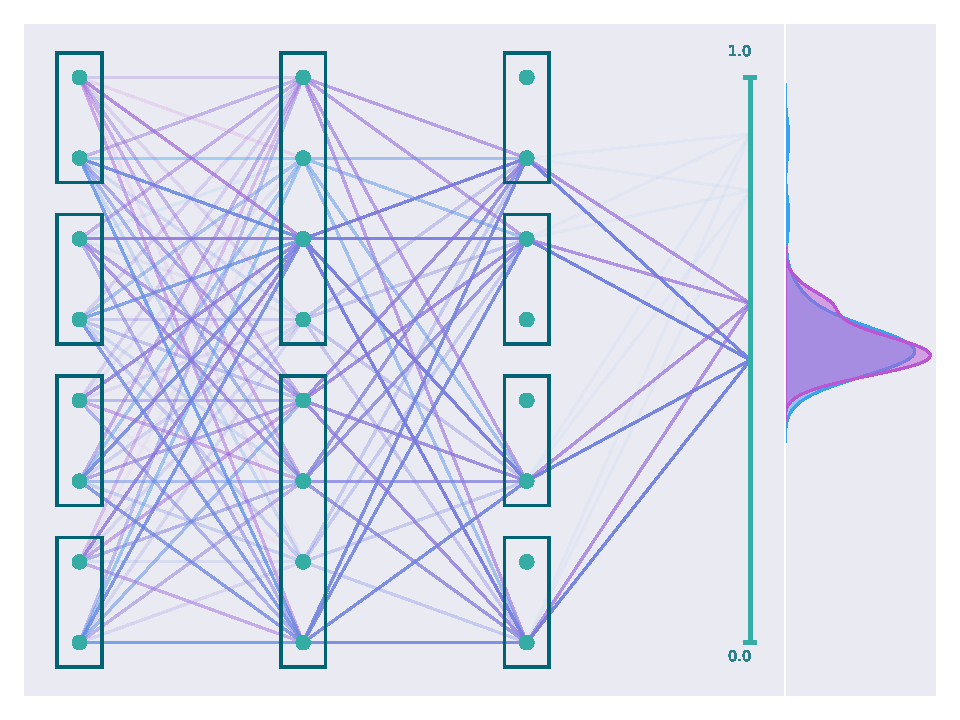
\includegraphics[width=\textwidth]{Figures/MLResults/NN/NetworkVis/BeforeTraining.pdf}
        \caption{}
        \label{fig:BTraining}
    \end{subfigure}
    \hfill
    \begin{subfigure}{.6\textwidth}
        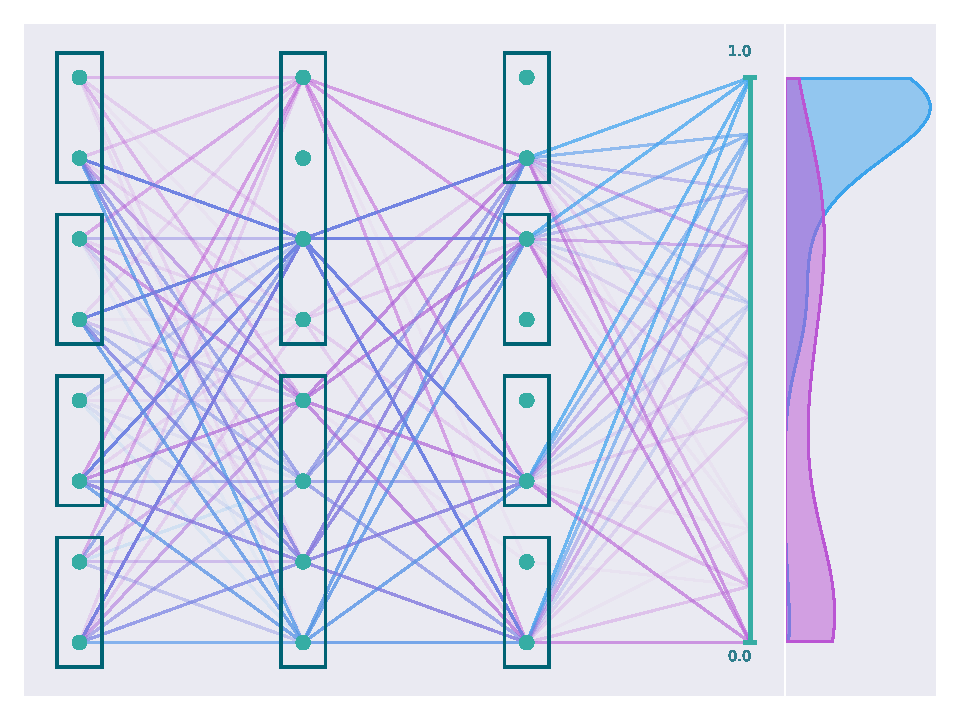
\includegraphics[width=\textwidth]{Figures/MLResults/NN/NetworkVis/AfterTraining.pdf}
        \caption{}
        \label{fig:ATraining}
    \end{subfigure}
    }
    \caption[A calculated visualization of the activation of a three layer maxout network, before and after training.]{
    A calculated visualization of a three layer maxout network. Each path 
    represents a data point where all connected nodes were the largest activation in their respective 
    unit. The distribution on the far right represent the output distribution. The figure to the left
    (\ref{fig:BTraining}) is the result before training and the figure to right (\ref{fig:ATraining})
    is after.}
\end{figure}
\begin{figure}
    \makebox[\linewidth][c]{%
    \centering
    \begin{subfigure}{.6\textwidth}
        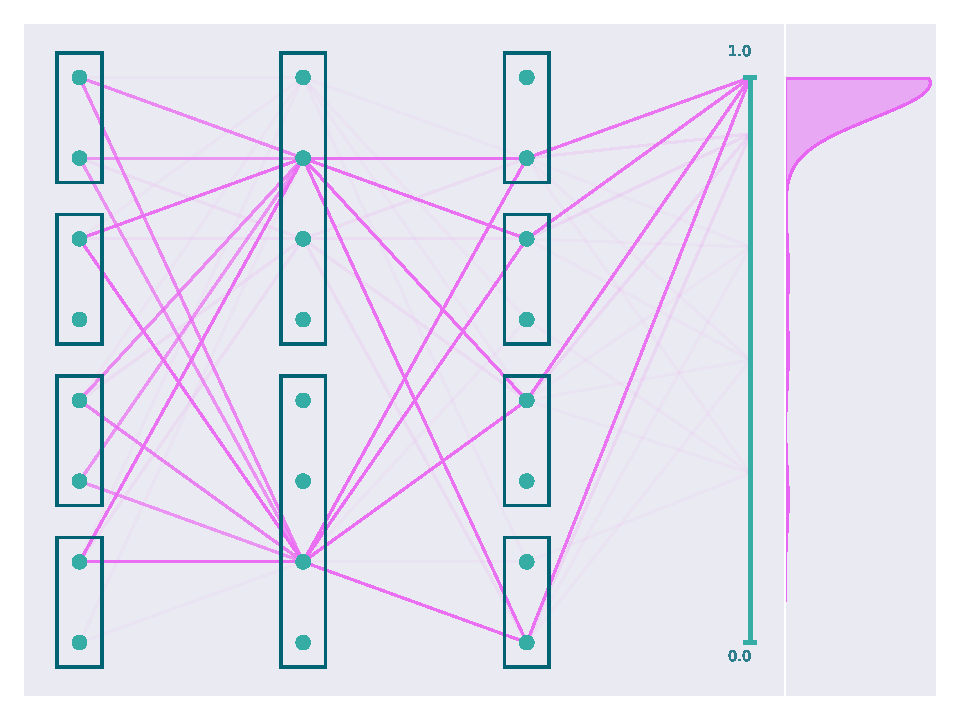
\includegraphics[width=\textwidth]{Figures/MLResults/NN/NetworkVis/AfterTrainingSig.pdf}
        \vspace{-0.5cm}
        \caption{}
        \label{fig:ATrainingSig}
    \end{subfigure}
    \hfill
    \begin{subfigure}{.6\textwidth}
        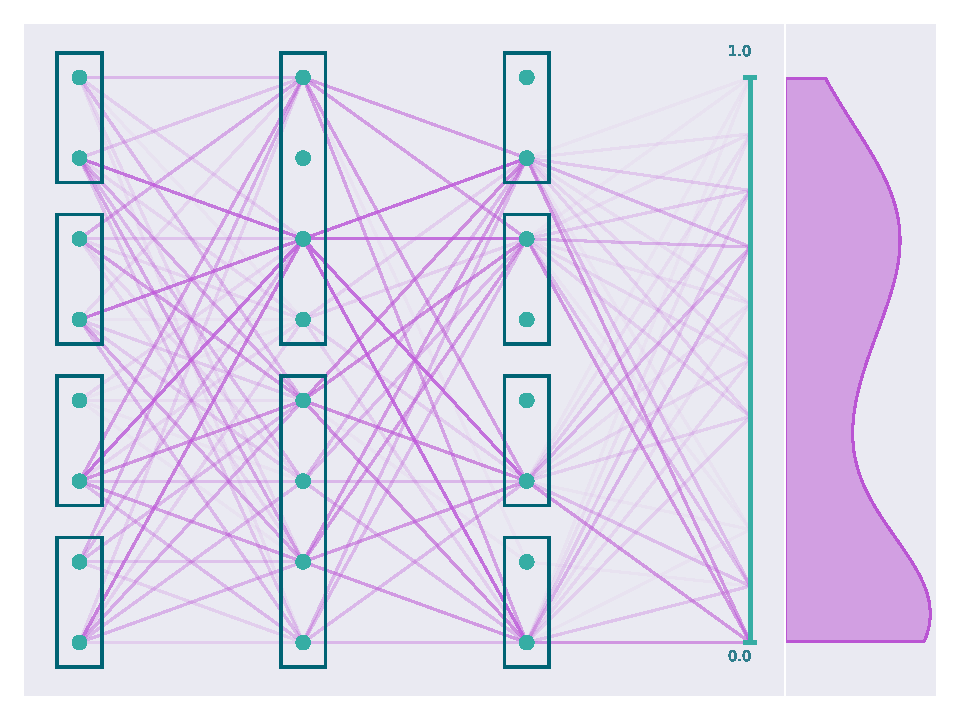
\includegraphics[width=\textwidth]{Figures/MLResults/NN/NetworkVis/AfterTrainingBkg.pdf}
        \vspace{-0.5cm}
        \caption{}
        \label{fig:ATrainingBkg}
    \end{subfigure}
    }
    \caption[A calculated visualization of the activation of a three layer maxout network, after training and displaying the
    signal and background separately.]{A calculated visualization of a three layer maxout network. The lines represent the path 
    through the nodes with the largest activation in their respective unit. The bolder the line the more frequently the path is 
    used. The distribution on the far right represent the output distribution and the figure with blue 
    paths (left) \ref{fig:ATrainingSig} is the result of signal, and the pink paths (right) is a result from background 
    \ref{fig:ATrainingBkg}.} 
    \label{fig:NetDist1}
\end{figure}

\begin{figure}
    \makebox[\linewidth][c]{%
    \centering
    \begin{subfigure}{.6\textwidth}
        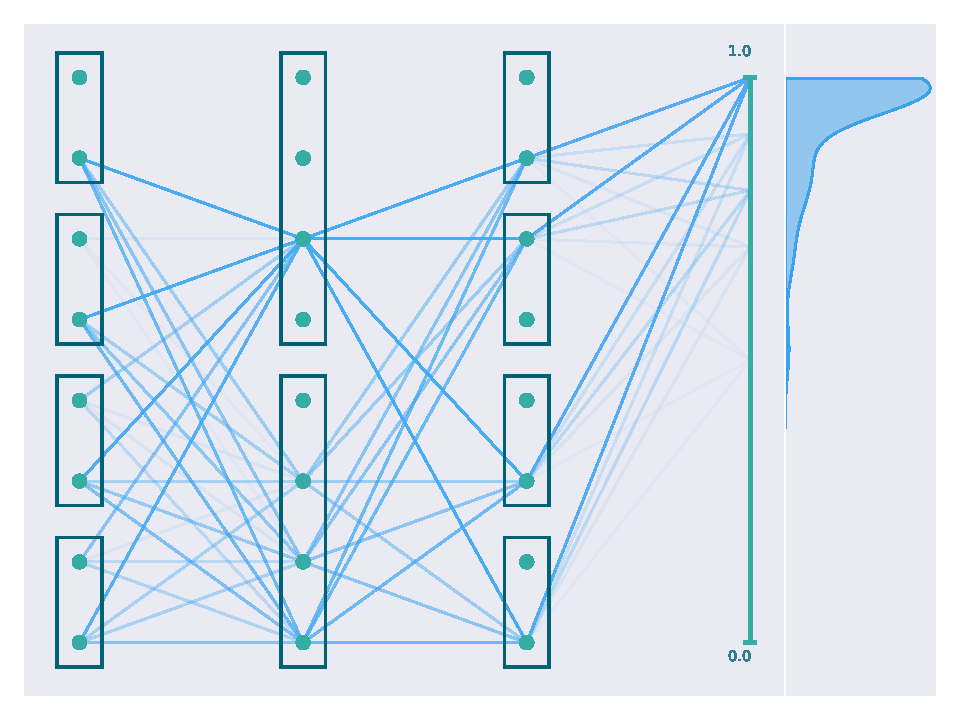
\includegraphics[width=\textwidth]{Figures/MLResults/NN/NetworkVis/AfterTrainingSig50250.pdf}
        \vspace{-0.5cm}
        \caption{}
        \label{fig:ATrainingSig50250}
    \end{subfigure}
    \hfill
    \begin{subfigure}{.6\textwidth}
        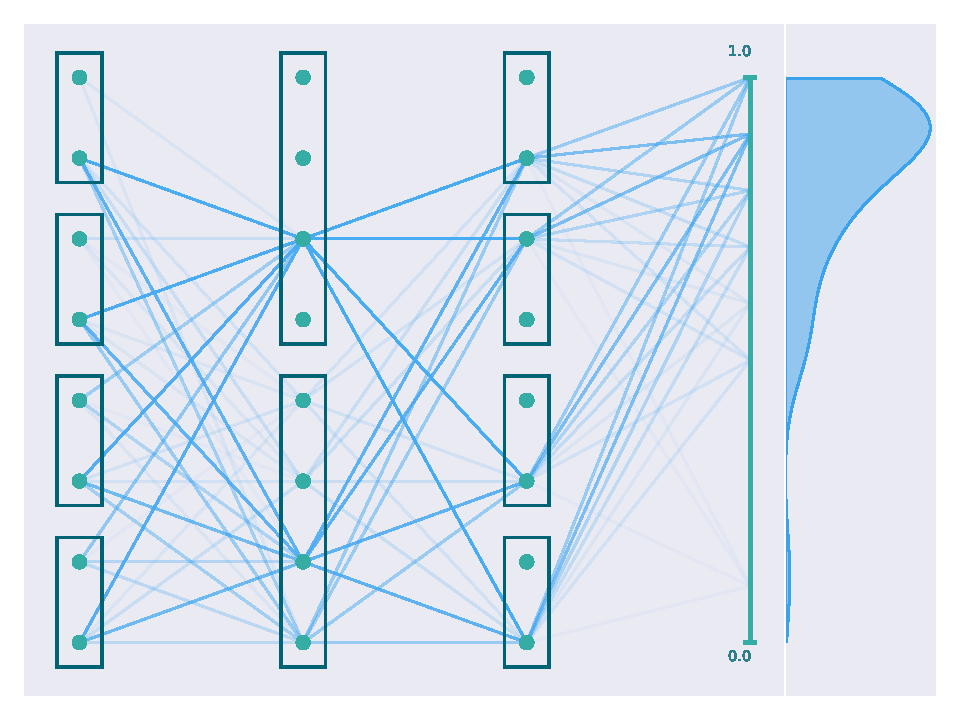
\includegraphics[width=\textwidth]{Figures/MLResults/NN/NetworkVis/AfterTrainingSig200300.pdf}
        \vspace{-0.5cm}
        \caption{}
        \label{fig:ATrainingSig200300}
    \end{subfigure}
    }
    \caption[A calculated visualization of the activation of a three layer maxout network, after training and displaying
    the results for two signal with each their own mass combination.]{A calculated visualization of a trained maxout network 
    with three hidden layers. The lines represent the path through the nodes with the largest activation in their respective
    unit. The bolder the line the more frequently the path is used. The distribution on the far right represent the output 
    distribution. The figure to the left (\ref{fig:ATrainingSig50250}) is a result of signal with masses $\{50,250\}_{GeV}$, 
    and the right (\ref{fig:ATrainingSig200300}) with masses $\{200,300\}_{GeV}$.}
    \label{fig:NetVisSigComp}
\end{figure}
Ideally, we would want the model to not only be able to separate the signal from the background, but do so in 
a way which allows the network to store the different patterns within the signal. In section \ref{subsubsec:Channel-Out},
I described this ability as long-term memory. One way to implement long-term memory is through a high number of parameters.
However through the \ac{LWTA} layers we can achieve the same through specific paths. To study this I have created similar 
figures as discussed in the paragraphs above, but this time only including results from applying the network on one mass combination. 
Figures \ref{fig:ATrainingSig50250} and \ref{fig:ATrainingSig200300} present the results for the mass combinations 
$\{50,250\}_{GeV}$, and $\{200,300\}_{GeV}$ respectively.
By comparing the figures, we see a small but noticeable difference in paths. Again the middle hidden layer seems to be 
the differentiating factor. To highlight the differences, I have included a cutout, comparing the first and second node in the bottom unit 
for the middle layer of both figures, \ref{fig:ATrainingSig50250Zoom} and \ref{fig:ATrainingSig200300Zoom}.
By studying the cutouts, we can discern that the maxout layer allows the model to discriminate both background from signal, 
and different variations of the signal through an increase in long-term memory. We can conclude that the maxout layer not only 
applies a form of regularization, but also increases the long-term memory of the model through pattern-specific paths through the network.\\
\begin{figure}
    \makebox[\linewidth][c]{%
    \centering
    \hfill
    \hfill
    \begin{subfigure}{.09\textwidth}
        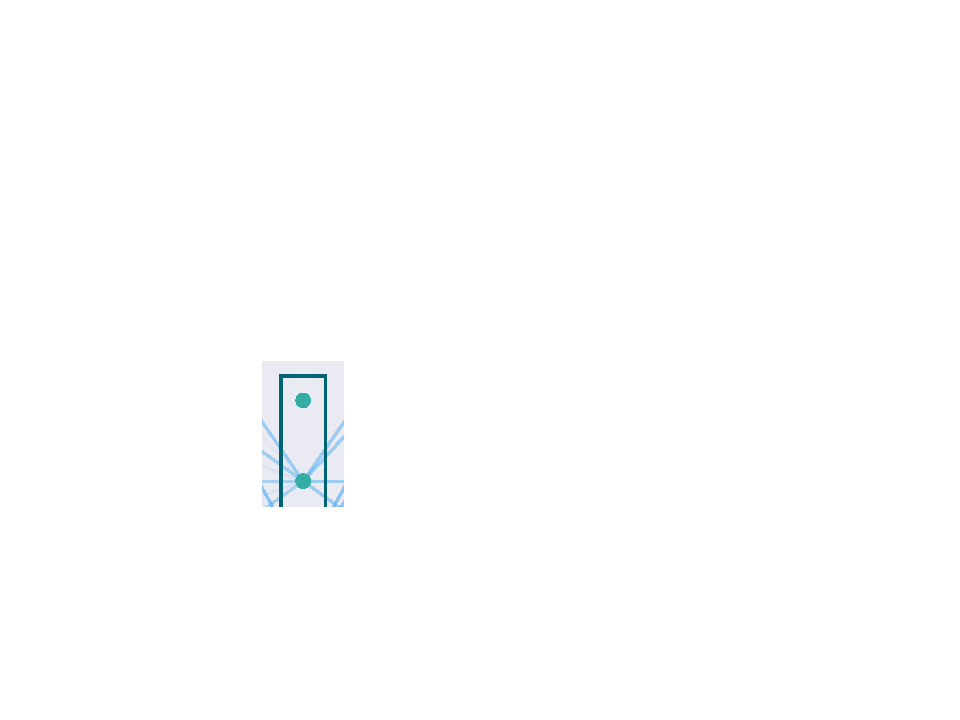
\includegraphics[width=\textwidth]{Figures/MLResults/NN/NetworkVis/AfterTrainingSig50250Zoom.pdf}
        \vspace{-0.5cm}
        \caption{}
        \label{fig:ATrainingSig50250Zoom}
    \end{subfigure}
    \hfill
    \begin{subfigure}{.094\textwidth}
        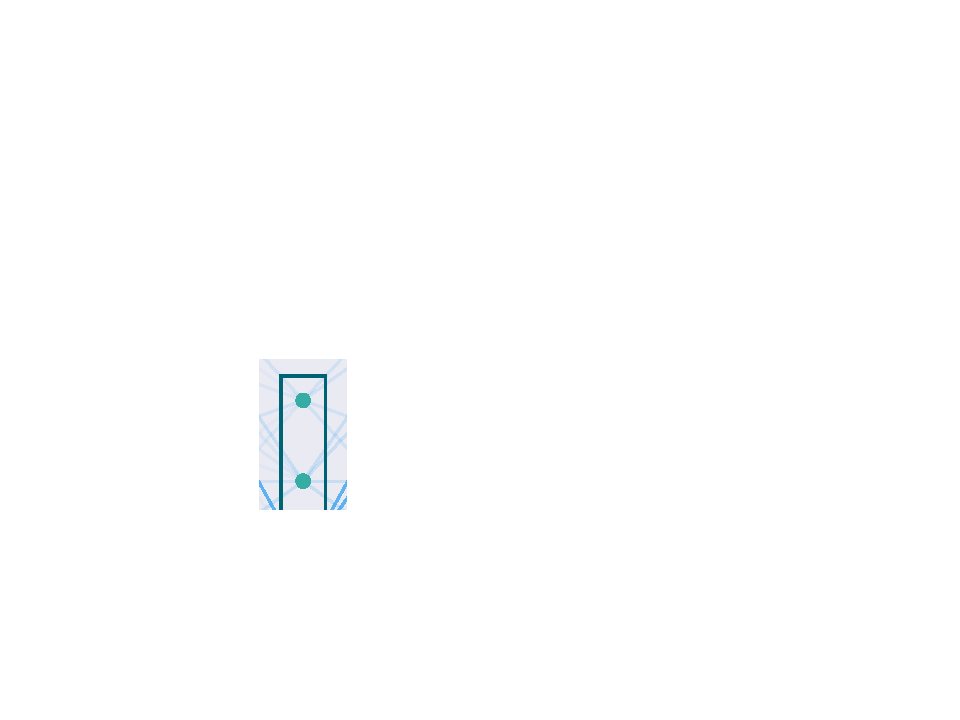
\includegraphics[width=\textwidth]{Figures/MLResults/NN/NetworkVis/AfterTrainingSig200300Zoom.pdf}
        \vspace{-0.5cm}
        \caption{}
        \label{fig:ATrainingSig200300Zoom}
    \end{subfigure}
    \hfill
    \hfill
    }
    \caption[A calculated visualization of the activation of a three layer maxout network, after training and displaying the
    the results for two signal with each their own mass combination, highlighting the difference between two specific nodes.]{
    A cut-out of the fifth and sixth node (counting from the top) in the second hidden layer, activated 
    by the signal with masses $\{50,250\}_{GeV}$ \ref{fig:ATrainingSig50250Zoom} and 
    $\{200,300\}_{GeV}$ \ref{fig:ATrainingSig200300Zoom}.}
    \label{fig:NetVisZoom}
\end{figure}
Finally, I wanted to compare the activations of the maxout model, to the activation of the \ac{SCO} model. In section \ref{subsubsec:stochchannelout},
I stated that the inspiration behind the \ac{SCO} was to elevate the channel-out method in a way which reduced complex co-adaptation among neighboring
nodes. In figure \ref{fig:NetDistSCO}, I included a visualization of the activation of a three layer \ac{SCO} network before (\ref{fig:BTrainingSCO}) 
and after (\ref{fig:ATrainingSCO}) training. However, it is important to note that the boxes in the figures do not equal the units given that the \ac{SCO} 
creates a large set of different units. The boxes are simply included for aesthetic reasons. By comparing the activations from the \ac{SCO} 
layers to maxout, we can discern that the \ac{SCO} behaves exactly as intended. In the figures visualizing the maxout layer (\ref{fig:NetDist1}), we can observe 
that several of the nodes which are not activated before training, are left dormant even after training. In comparison, the \ac{SCO} layers display a far more balanced 
activation, and exhibits no signs of complex co-adaptation. 
\begin{figure}[H]
    \makebox[\linewidth][c]{%
    \centering
    \begin{subfigure}{.6\textwidth}
        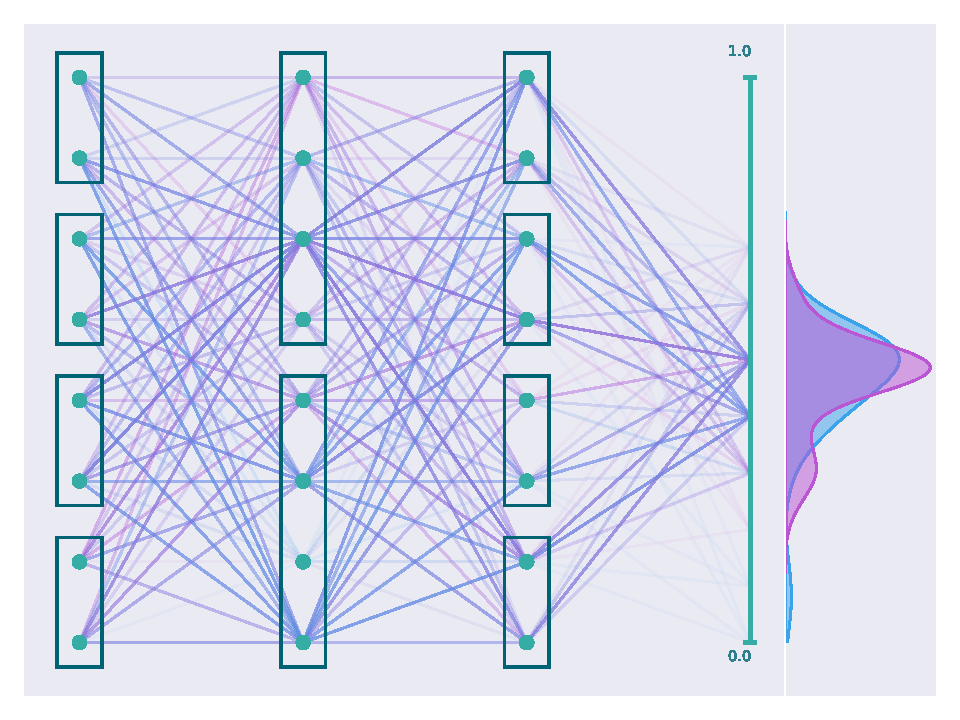
\includegraphics[width=\textwidth]{Figures/MLResults/NN/NetworkVis/SCO/BeforeTraining.pdf}
        \caption{}
        \label{fig:BTrainingSCO}
    \end{subfigure}
    \hfill
    \begin{subfigure}{.6\textwidth}
        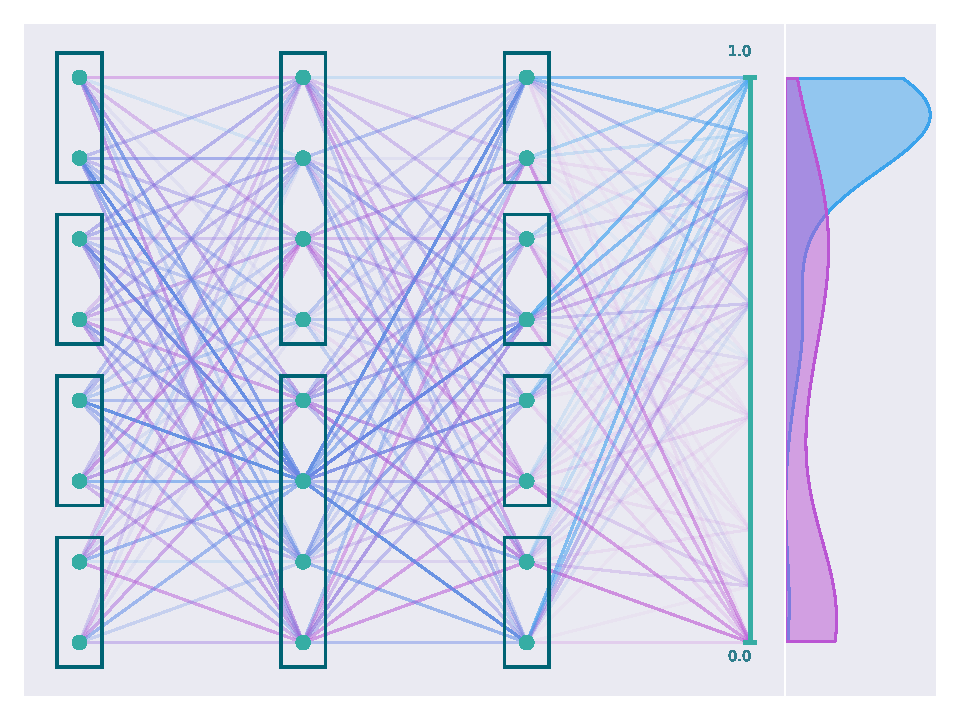
\includegraphics[width=\textwidth]{Figures/MLResults/NN/NetworkVis/SCO/AfterTraining.pdf}
        \caption{}
        \label{fig:ATrainingSCO}
    \end{subfigure}
    }
    \caption[A calculated visualization of the activation of a three layer \acs{SCO} network, after training and displaying the
    signal and background separately.]{A calculated visualization of a three layer \acs{SCO} network. The lines represent the path 
    through the nodes with the largest activation in their respective unit. The bolder the line the more frequently the path is used. 
    The distribution on the far right represent the output distribution. The figure to the left (\ref{fig:BTrainingSCO}) is the result 
    before training and the figure to right (\ref{fig:ATrainingSCO}) is after. Note: The boxes in the figures do \emph{not} represent the units, 
    given that the \ac{SCO} changes the units dynamically.} 
    \label{fig:NetDistSCO}
\end{figure}
\subsection{Training History and Overfitting}\label{subsec:Overfitting}
In section \ref{sec:Regularization} I described how creating ensembles of networks is a form of regularization. Therefore,
it is of interest to study the relationship between performance on the training set and the validation set for our ensemble 
methods. In figure \ref{fig:History} I drew plots displaying the performance using the original signal on the training and validation 
set after each epoch (50 in total), as measured in \ac{AUC} for both a dense \ac{NN} (\ref{fig:NNHist}) and maxout (\ref{fig:MaxOutHist}).
\\ 
In figure \ref{fig:NNHist} we can observe that an ordinary dense \ac{NN} reaches a maximum in performance for the validation set after only 
a couple of epochs. This peak is then followed by a quick drop in performance, while the training set increases in performance. 
The drop in performance for the validation set and increase in performance for the training set is a sure sign of overfitting. 
\\
In figure \ref{fig:MaxOutHist} we observe that an ensemble method (in this case the maxout) displays a different training history. For the first 
10 epochs the model increases in performance for both data sets. After this, the validation set does not decrease in performance, but 
simply holds stable while the training set increases. This is a sign that the model is not experiencing overfitting. Furthermore, the 
training history of the maxout model raises an interesting point. From experience I know that the maxout model reaches a peak in performance
on the validation set after approximately 15-20 epochs. Given that the performance after this is stable, it is plausible that continuing 
training will not worsen the performance or lead to overfitting, but rather improve. This is definitely an interesting possibility
for the \ac{LWTA} layers, but will not be studied in this thesis due to time constraints.
\\
In section \ref{subsec:TrainingStrategy}, I discussed the training strategy used when training all models in this analysis. I mentioned 
the implementation of an early stopping criterion which makes sure that the model continues to train only as long as the performance on the 
validation data set increases. By studying the subfigures in figure \ref{fig:History}, we can deduce that the ensemble methods will not only 
be able to avoid overfitting, but will as a consequence be allowed to train much longer than the other models.
\begin{figure}[H]
    \makebox[\linewidth][c]{%
    \centering
    \begin{subfigure}{.45\textwidth}
        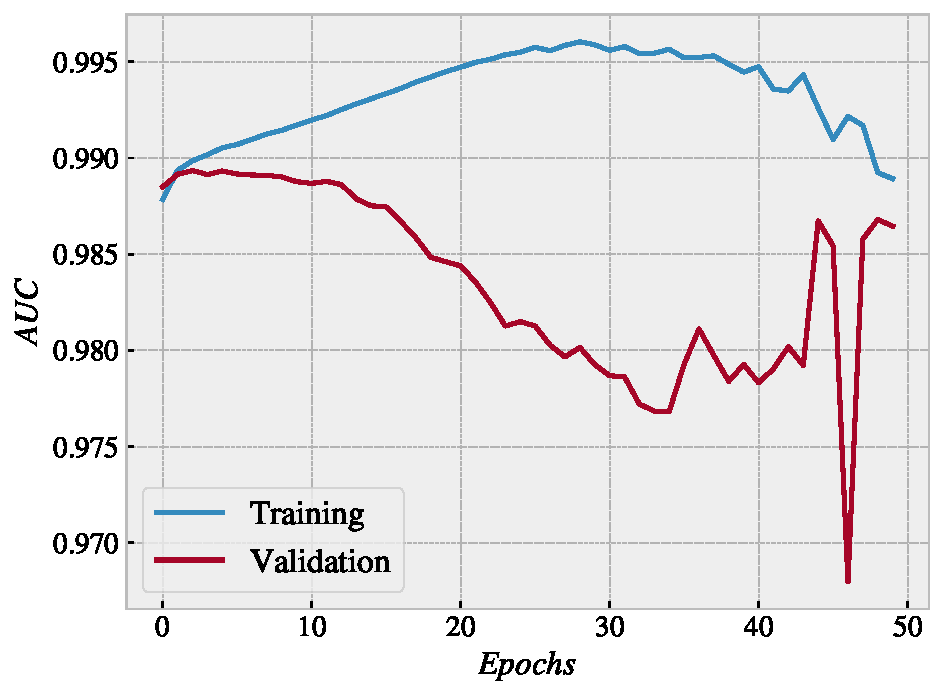
\includegraphics[width=\textwidth]{Figures/MLResults/NN/SUSY/History/NNHistory.pdf}
        \caption{}
        \label{fig:NNHist}
    \end{subfigure}
    \begin{subfigure}{.45\textwidth}
        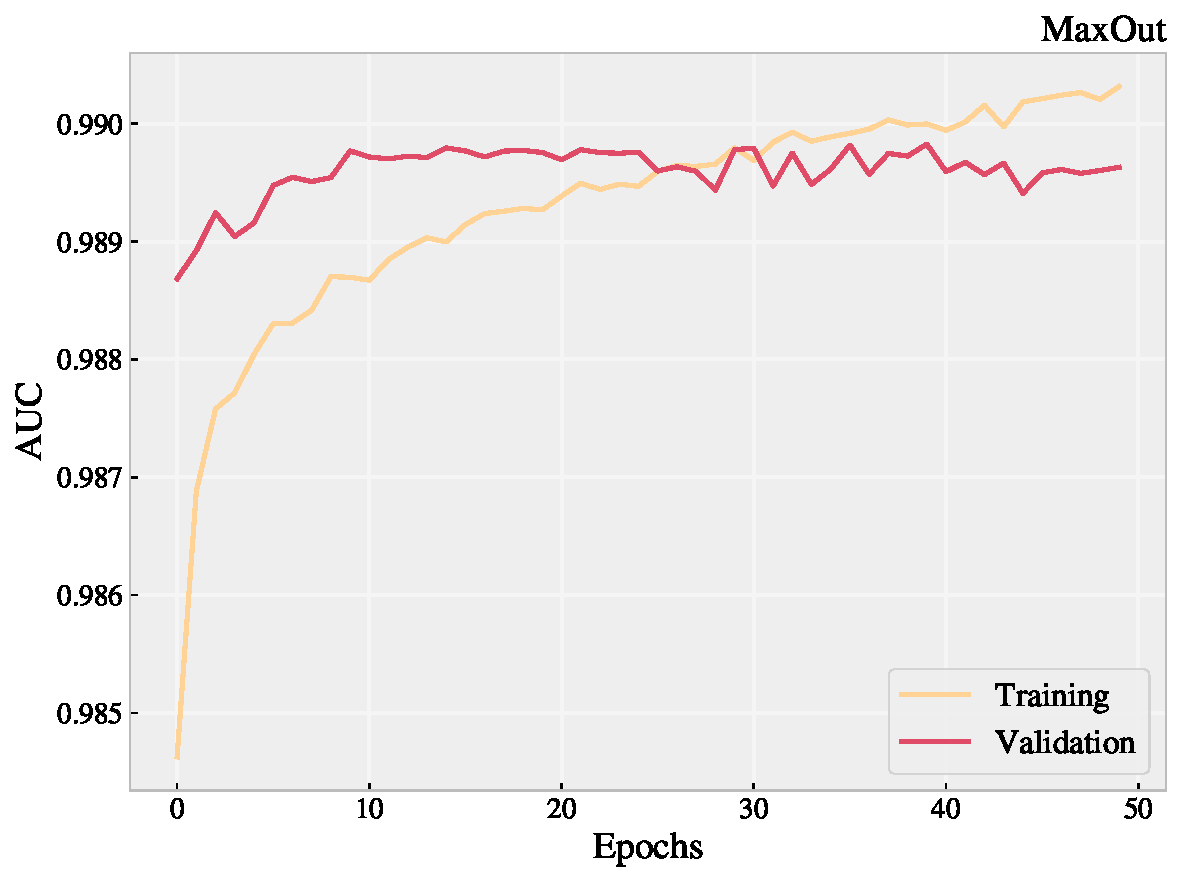
\includegraphics[width=\textwidth]{Figures/MLResults/NN/SUSY/History/MaxOutHistory.pdf}
        \caption{}
        \label{fig:MaxOutHist}
    \end{subfigure}
    }
    \caption[A plot comparing the \acs{AUC} score made after each epoch on both the training and validation set, between a dense \acs{NN} 
    and maxout model.]{A plot displaying the \acs{AUC} score made after each epoch on both the training and validation set. 
    Figure \ref{fig:NNHist} shows the results from the dense \ac{NN} and figure \ref{fig:MaxOutHist} shows
    the results from a maxout network.}
    \label{fig:History}
\end{figure}
\subsection{Comparing Achieved Sensitivity between Ensemble Methods}
In this section I will present and discuss the performance of the three different networks discussed in section 
\ref{subsec:Ensembles}, channel-out, \ac{SCO} and maxout. The results presented in this section were made using the
original signal set (see section \ref{subsec:signal}), the training strategy described in section \ref{subsec:TrainingStrategy}
and the architectures described in section \ref{subsec:arch}.
\\
In figure \ref{fig:MaxOutGridSig} I present the achieved sensitivity of the maxout model using the original signal set. 
The grid shows the same trends as the previous models, i.e. the preference in the higher statistics mass combinations. By comparing 
the results from the maxout model to the deep, dense network presented in figure \ref{fig:NNGridSig}, we discern that the dense 
network outperforms the maxout model (ever so slightly) for the higher statistic mass combinations. It is plausible that this is due 
to the difference in depth. The dense network utilizes 3 hidden layers of 600 nodes each, while the maxout, although built with the 
same architecture, only utilizes 200 nodes per layer when propagating input through the network. This could result in the dense network 
being able to more deeply tune for the patterns in the higher statistics combinations.
\\
However, the most interesting result for the maxout model, is its ability to tune for all mass combinations. Although the dense network
outperformed the maxout model for the high statistics combinations, the maxout model outperformed the dense for most other combination (26 of 
the 30 possible mass points). This result can be credited to two factors. The first being maxout's effect as a form of regularization. In the previous 
section (see section \ref{subsec:Overfitting}), I presented how, maxout, through its regularization abilities, is able to 
uphold the early stopping criteria for a larger number of epochs. The second factor is maxout's innate long-term memory which was studied
in section \ref{subsec:Viz}. From figure \ref{fig:MaxOutGridSig}, we are able to deduce that although the maxout model is not able to tune 
to the same depth for the lower masses, it is able to achieve a large level of generalizability through reducing overfitting and increasing 
long-term memory.\\
\begin{figure}
    \makebox[\linewidth][c]{%
    \centering
    \begin{subfigure}{.65\textwidth}
        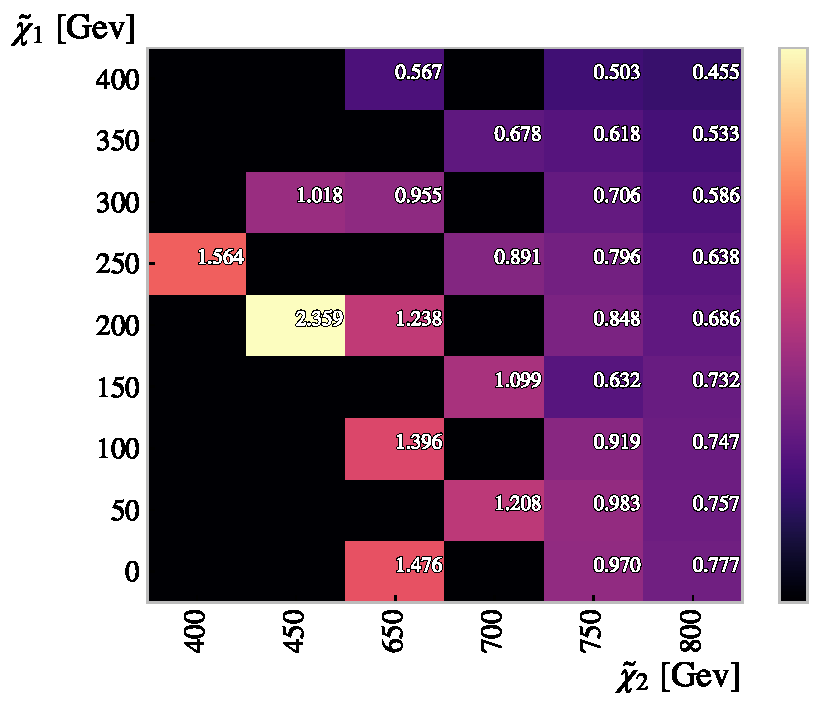
\includegraphics[width=\textwidth]{Figures/MLResults/NN/SUSY/Grid/MaxOutGridSig.pdf}
    \end{subfigure}
    }
    \caption{A grid displaying the expected significance on the original signal set using the signal region 
    created by the maxout network.}
    \label{fig:MaxOutGridSig}
\end{figure}
In appendix \ref{appendix:Ensembles} I have included grids displaying the achieved sensitivity for both channel-out and \ac{SCO}. Both 
models demonstrate similar performance to the maxout layer. To compare the three methods I created a 'pie-plot'. A 'pie-plot' 
compares the achieved sensitivity between several models and displays the results for each individual mass combination.  In figure 
\ref{fig:EnsembleComp} I present the 'pie-plot' comparing maxout, channel-out and \ac{SCO}. Each mass combination includes a 'pie', where 
the size of each 'slice' represents the relative size of the significance compared to the other methods. For example, if a slice occupies 
half of the 'pie', then the method corresponding to that slice achieved a significance equal to the sum of the significance of the other methods.
The color surrounding each 'pie' marks which method achieved the highest sensitivity for the respective combination.
\\
By studying the 'pie-plot' in figure \ref{fig:EnsembleComp}, we can deduce that maxout model outperforms the other two in most of the mass 
combination (24 out of the 30 mass points). From the sizes of each slice, we can deduce that all three models seem relatively equal in performance, maxout 
only outperforming the others by a small fraction. The most interesting observation from the 'pie-plot' is the performance from the \ac{SCO}, as 
this model was in-part created by me. Except the mass combinations where maxout was the most sensitive, \ac{SCO} was the best performing model. 
Most interestingly, it outperformed the channel-out model, which is the model most similar to \ac{SCO}, in 9 out of the 30 mass point (see figure \ref{fig:SCOCO}). 
In hindsight, I believe that by removing the \ac{SCO} during prediction (similar to what is done for dropout), the \ac{SCO} layer would greatly 
improve in performance, on a count of the fact that the performance on each event is dependent on the random choice of unit for that prediction.
This means it is possible that upon prediction, a data point is sent through a path which has never been chosen during training. 
Nonetheless, this analysis is an indicator that although the maxout model was the highest performing model, the \ac{SCO} layer shows 
great promise and should be further explored in further analysis. 
\begin{figure}
    \makebox[\linewidth][c]{%
    \centering
    \begin{subfigure}{.75\textwidth}
        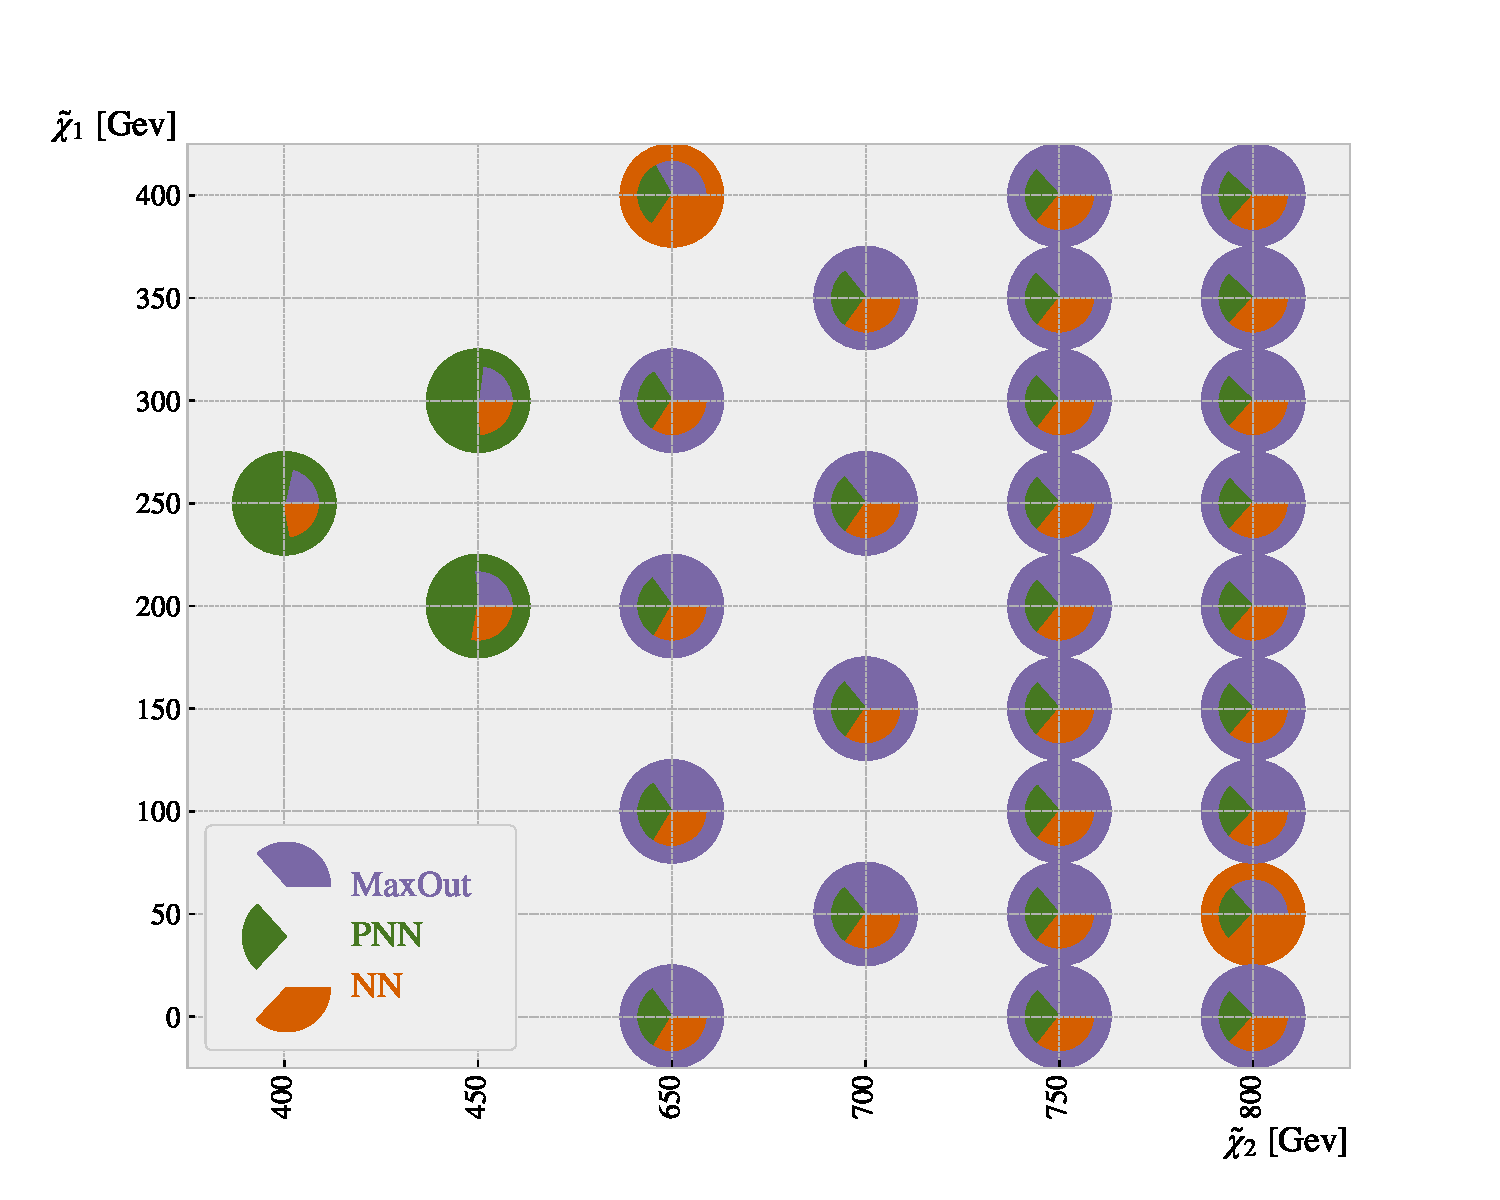
\includegraphics[width=\textwidth]{Figures/MLResults/NN/SUSY/Comparison/EnsemblesNetworkComp.pdf}
    \end{subfigure}
    }
    \caption[A sensitivity comparison between the ensemble networks (maxout, \acs{SCO}, channel-out) on the original 
    signal data.]{A sensitivity comparison between the ensemble networks (maxout, \acs{SCO}, channel-out) on the original 
    signal data. The size of each slice represents the relative size of the significance and the color around each 
    point displays the method with the largest sensitivity for the respective combination.}
    \label{fig:EnsembleComp}
\end{figure}

